\documentclass[tikz,border=10pt]{standalone}
\usepackage{xcolor}
\usepackage{newpxtext}
\usepackage{tikz}
\usetikzlibrary{shapes.geometric, arrows.meta, positioning, calc, fit, backgrounds}

% Color Palette matching template.tex
\definecolor{SitePrimary}{RGB}{165, 124, 117}
\definecolor{DarkCharcoal}{HTML}{2B2B2B}
\definecolor{LightTaupe}{RGB}{245, 242, 240}
\definecolor{SubtleGray}{HTML}{F4F4F4}
\definecolor{BoxBorder}{HTML}{D0C9C5}
\definecolor{AccentGreen}{HTML}{2E7D32}
\definecolor{AccentRed}{HTML}{C62828}

\begin{document}
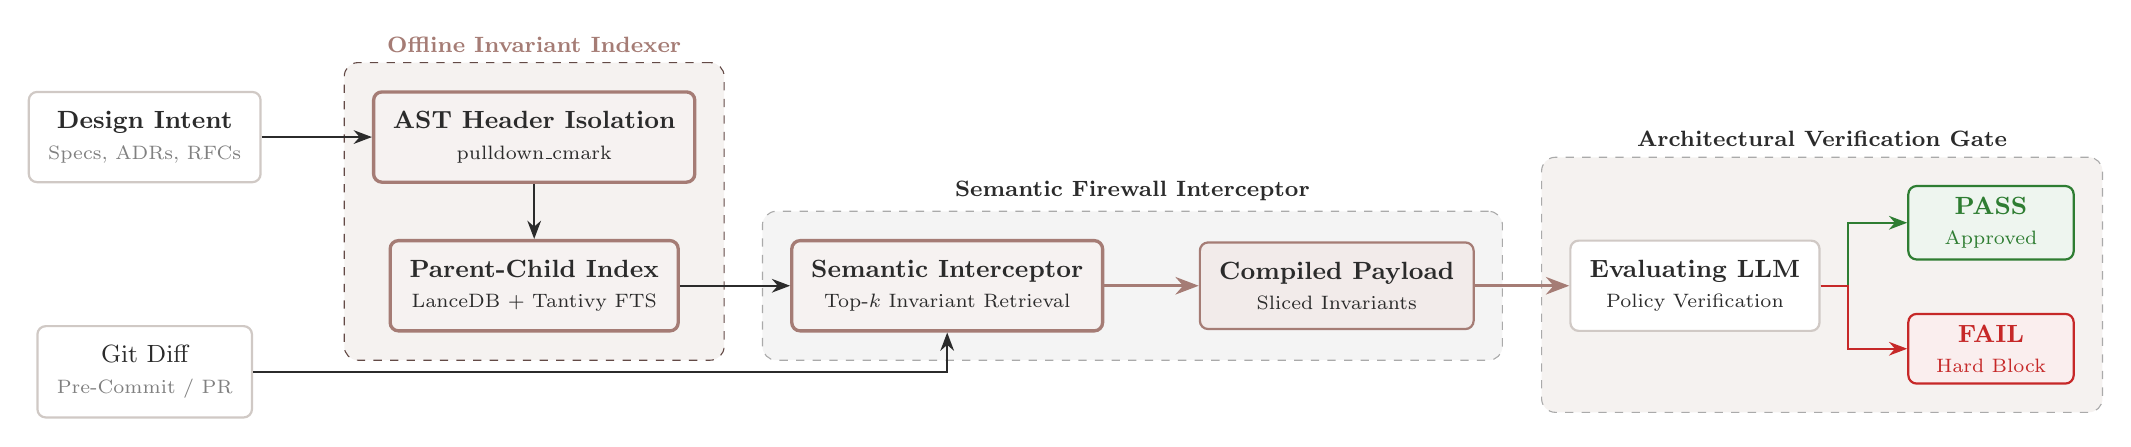
\begin{tikzpicture}[
    font=\small\color{DarkCharcoal},
    >=Stealth,
    node distance=1.8cm and 1.2cm,
    decisionblock/.style={
        rectangle,
        rounded corners=3pt,
        thick,
        align=center,
        inner sep=4pt,
        minimum height=0.75cm,
        minimum width=2.1cm
    },
    block/.style={
        rectangle,
        draw=BoxBorder,
        fill=white,
        rounded corners=3pt,
        thick,
        align=center,
        inner sep=7pt,
        minimum height=1.1cm,
        minimum width=2.4cm
    },
    primaryblock/.style={
        rectangle,
        draw=SitePrimary,
        fill=SitePrimary!10!white,
        rounded corners=3pt,
        very thick,
        align=center,
        inner sep=7pt,
        minimum height=1.1cm,
        minimum width=2.4cm
    },
    subgraph/.style={
        draw=SitePrimary!60!black,
        fill=LightTaupe,
        rounded corners=5pt,
        dashed,
        inner sep=10pt
    },
    line/.style={
        ->,
        thick,
        color=DarkCharcoal
    },
    highlightline/.style={
        ->,
        very thick,
        color=SitePrimary
    },
    badge/.style={
        fill=SitePrimary,
        text=white,
        font=\scriptsize\bfseries,
        rounded corners=2pt,
        inner sep=2pt
    }
]

    % --- Nodes: Column 1 (Inputs) ---
    \node[block] (docs) {\textbf{Design Intent}\\{\scriptsize\color{gray}Specs, ADRs, RFCs}};
    \node[block, below=1.8cm of docs] (gitdiff) {Git Diff\\{\scriptsize\color{gray}Pre-Commit / PR}};

    % --- Nodes: Column 2 (Engine Core) ---
    \node[primaryblock, right=1.4cm of docs] (ast) {\textbf{AST Header Isolation}\\{\scriptsize pulldown\_cmark}};
    \node[primaryblock, below=0.7cm of ast] (lancedb) {\textbf{Parent-Child Index}\\{\scriptsize LanceDB + Tantivy FTS}};
    
    % --- Nodes: Column 3 (Interceptor) ---
    \node[primaryblock, right=1.4cm of lancedb] (query) {\textbf{Semantic Interceptor}\\{\scriptsize Top-$k$ Invariant Retrieval}};
    \node[block, fill=SitePrimary!15!white, draw=SitePrimary, right=1.2cm of query] (payload) {\textbf{Compiled Payload}\\{\scriptsize Sliced Invariants}};

    % --- Nodes: Column 4 (Model & Decision) ---
    \node[block, right=1.2cm of payload] (llm) {\textbf{Evaluating LLM}\\{\scriptsize Policy Verification}};
    \node[decisionblock, right=1.1cm of llm, text=AccentGreen, draw=AccentGreen, fill=AccentGreen!8!white, yshift=0.8cm] (pass) {\textbf{PASS}\\{\scriptsize Approved}};
    \node[decisionblock, right=1.1cm of llm, text=AccentRed, draw=AccentRed, fill=AccentRed!8!white, yshift=-0.8cm] (fail) {\textbf{FAIL}\\{\scriptsize Hard Block}};

    % --- Subgraph Backgrounds ---
    \begin{scope}[on background layer]
        \node[subgraph, fit=(ast) (lancedb), label={[font=\footnotesize\bfseries\color{SitePrimary}, anchor=south]north:Offline Invariant Indexer}] (enginebox) {};
        \node[subgraph, fit=(query) (payload), fill=SubtleGray, draw=DarkCharcoal!40, label={[font=\footnotesize\bfseries\color{DarkCharcoal}, anchor=south]north:Semantic Firewall Interceptor}] (firewallbox) {};
        \node[subgraph, fit=(llm) (pass) (fail), fill=LightTaupe, draw=DarkCharcoal!40, label={[font=\footnotesize\bfseries\color{DarkCharcoal}, anchor=south]north:Architectural Verification Gate}] (verifybox) {};
    \end{scope}

    % --- Connections ---
    \draw[line] (docs) -- (ast);
    \draw[line] (ast) -- (lancedb);
    \draw[line] (lancedb) -- (query);
    \draw[line] (gitdiff.east) -| (query.south);
    \draw[highlightline] (query) -- (payload);
    \draw[highlightline] (payload) -- (llm);
    \draw[line, color=AccentGreen] (llm.east) -- ++(0.35cm,0) |- (pass.west);
    \draw[line, color=AccentRed] (llm.east) -- ++(0.35cm,0) |- (fail.west);

\end{tikzpicture}
\end{document}
